\documentclass[11pt,reqno,final]{amsart}

\pdfcompresslevel=0
\pdfobjcompresslevel=0

\usepackage[dvipsnames]{xcolor}% adds colors
\usepackage{amsmath, amsthm}% {amsfonts, amssymb}

% New Characters
\usepackage[latin1]{inputenc}%
\usepackage[T1]{fontenc}

\usepackage{MnSymbol}
\usepackage[normalem]{ulem}% underlining

\usepackage[theoremfont, largesc]{newpxtext} % different text,math font
\usepackage{newpxmath}

\makeatletter
\DeclareMathRadical{\sqrtsign}{symbols}{112}{largesymbols}{112}
% \let\sqrt=\undefined
% \DeclareRobustCommand\sqrt{\@ifnextchar[\@sqrt{\mathpalette\@x@sqrt}]}
% \def\@x@sqrt#1#2{%
%  \setbox\z@\hbox{$\m@th#1\sqrtsign{\mkern1mu #2}$}
%  \mkern3mu\box\z@}
\makeatother




% Page Typesetting
\usepackage[final]{microtype}
\usepackage{relsize}
\usepackage[margin=1in]{geometry}
\usepackage{framed}
\usepackage{tikz}

\usepackage{csquotes}

\usepackage{setspace}
\onehalfspacing

\usepackage{hyperref}
\hypersetup{
  final,
  pdftitle={Math 135 - Implicit Differentiation},
  pdfauthor={Bonventre}, 
  linktoc=page,
  pagebackref,
  colorlinks=true,
  citecolor=PineGreen,
  linkcolor=PineGreen,
  linkbordercolor=PineGreen,
}


% Internal References

\usepackage[inline,shortlabels]{enumitem}

% \numberwithin{equation}{section} 
\numberwithin{figure}{section}

\usepackage[nameinlink,capitalise,noabbrev]{cleveref}

\crefname{equation}{}{} % get \cref to behave as \eqref

% \theoremstyle{plain} % bold name, italic text
\newtheorem{theorem}[equation]{Theorem}%
\newtheorem*{theorem*}{Theorem}%
\newtheorem{lemma}[equation]{Lemma}%
\newtheorem{proposition}[equation]{Proposition}%
\newtheorem{corollary}[equation]{Corollary}%
\newtheorem{conjecture}[equation]{Conjecture}%
\newtheorem*{conjecture*}{Conjecture}%
\newtheorem{claim}[equation]{Claim}%
\newtheorem{question}{Question}

\theoremstyle{definition} % bold name, plain text
\newtheorem{definition}[equation]{Definition}%
\newtheorem*{definition*}{Definition}%
\newtheorem{example}[equation]{Example}%
\newtheorem*{example*}{Example}%
\newtheorem{remark}[equation]{Remark}%
\newtheorem{notation}[equation]{Notation}%
\newtheorem{convention}[equation]{Convention}%
\newtheorem{assumption}[equation]{Assumption}%
\newtheorem{exercise}[question]{Exercise}

% ---------- macros
\newcommand{\set}[1]{\left\{#1\right\}}%
\newcommand{\sets}[2]{\left\{ #1 \;|\; #2\right\}}%
\newcommand{\longto}{\longrightarrow}%
\newcommand{\into}{\hookrightarrow}%
\newcommand{\onto}{\twoheadrightarrow}%

\usepackage{harpoon}
\newcommand{\vect}[1]{\text{\overrightharp{\ensuremath{#1}}}}

\newcommand{\del}{\partial}%

\newcommand{\ki}{\chi}
\newcommand{\ksi}{\xi}
\newcommand{\Ksi}{\Xi}

\newcommand{\dlim}{\displaystyle\lim}

% %%%%%%%%%%%%%%%%%%%%%%%%%%%%%%%%%%%%%%%%%%%%%%%%%%%%%%%%%%%%%%%%%%%%%%%%%%%%%%%%%%%%%%%%%%%%%%%%%%%%

\begin{document}


\begin{center}
        \textbf{\Large Math 135, Calculus 1, Fall 2020}\\[10pt]
        {\large 10-22: Implicit Differentiation (Section 3.8)}
\end{center}

\thispagestyle{empty}


\renewcommand{\thesection}{\Alph{section}}

% \vspace{-1pt}

The \textbf{derivative} $f'(x)$ of a function $f(x)$ gives:
\begin{itemize}
\item the slope of the tangent line
\item the instantaneous velocity
\item the instantaneous rate of change
\end{itemize}


\section{Chain Rule}

The chain rule gives us a way to compute the derivative of a \textbf{composite} of two functions.
\begin{theorem*}
        If $O(x)$ and $I(x)$ are differentiable functions, then so is the composite $O(I(x)) = (O \circ I)(x)$.
        Moreover,
        \begin{framed}
                \[
                        \dfrac{d}{dx}\Big( O(I(x)) \Big) = O'\big( I(x) \big) \cdot I'(x).
                \]
        \end{framed}
\end{theorem*}

\begin{exercise}
        Compute $\dfrac{d}{dx} \Big( \sin\left(e^{\sqrt{2x}}\right) \Big)$.
        \vfill
\end{exercise}

\section{Implicit Differentiation}

If $y$ and $x$ are related not by a function, but by a general equation such as
\[
        y^4+xy = x^3 - x + 2,
\]
we should still be able to compute the function $\dfrac{dy}{dx}$, the slope of the tangent line at a point.
\begin{center}
        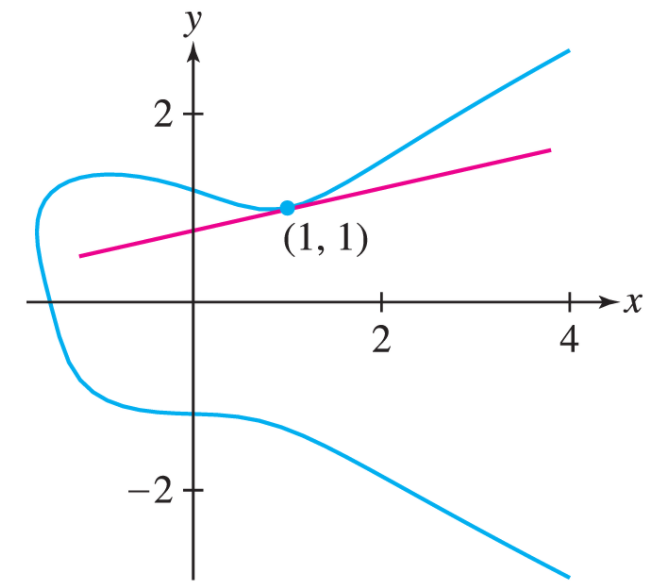
\includegraphics[width=2.5in]{10-23P_dydx.png}
\end{center}

\newpage

\begin{example}
        To compute $\dfrac{dy}{dx}$ for $x+^2 + y^2  = 2x$,
        we take the derivative of both sides of the equation with respect to $x$:
        \begin{align*}
          \dfrac{d}{dx}(x^2 + y^2) &= \dfrac{d}{dx}(2x)\\
          2x + \dfrac{d}{dx}(y^2) &= 2
        \end{align*}
        To compute $\dfrac{d}{dx}(y^2)$, we use the Chain Rule: we think of $y$ as representing a function $y = y(x)$ of $x$,
        and then the chain rule says
        \[
                \dfrac{d}{dx}(y^2) = \dfrac{d}{dx}(y(x)^2) = 2 \cdot y(x) \cdot y'(x) = 2y\dfrac{dy}{dx}.
        \]
        All together, we have
        \[
                2x + 2y\dfrac{dy}{dx} = 2,
        \]
        and solving for $\dfrac{dy}{dx}$ (and assuming $y \neq 0$) we get
        \[
                \dfrac{dy}{dx} = \dfrac{1 - x}{y}.
        \]
\end{example}

\begin{exercise}
        Use the Product Rule to compute $\dfrac{d}{dx}(xy)$.
        \vfill
\end{exercise}

\begin{exercise}
        Use the Quotient Rule to compute $\dfrac{d}{dx}\left( \dfrac{y}{x} \right)$.
        \vfill
\end{exercise}

\newpage

\begin{exercise}
        Compute $\dfrac{dy}{dx}$ if $\sin(xy) = y^2$.
        \vfill
\end{exercise}

\begin{exercise}
        Compute $\dfrac{dy}{dx}$ if $e^x + e^y = xy$.
        \vfill
\end{exercise}

\begin{exercise}
        Find the slope of the tangent line to the graph of $e^y\sin(x) = 1$ at $(\pi/2, 0)$.
        \vfill
\end{exercise}


\end{document}
